\section{SIMP Implementation in Julia}

The SIMP algorithm consists of two main loops. The inner loop consists of the optimization process facilitated by the Method of Moving Asymptotes while the outer loop increases the penalization parameter $p$ after each inner loop has completed. The whole process is repeated until a desired threshold is met, such as a small enough norm between successive minimal objective function evaluations. The algorithm implementation in the Julia language can be found in \ref{sec:SIMP-Alg} and is available for download on \href{https://github.com/mikwnelson/julia-simp-optimization}{GitHub}.

Figure \ref{fig:SIMP-Outputs-20-40-60} shows design results for domains of varying numbers of control volumes. Notice in Figures \ref{fig:SIMP-Output-40} and \ref{fig:SIMP-Output-60} that the ends of the ``tentacles'' contain some control volumes with $\eta\neq 1$. This is due to the cap put on $p$ in the algorithm. It became necessary to impose a maximum value for $p$ as the number of control volumes increased in order to complete the algorithm within a reasonable amount of time. With higher resolutions (i.e. more control volumes), it appears that the algorithm continuously is trading high conductivity material between the ends of the symmetric branches above and below the horizontal midline.

It is interesting to note the symmetry in the designs. In \cite{Marck2012} the authors chose to take advantage of this symmetry and compute only the upper half of the domain and then reflect that design across the central horizontal axis. While \ref{fig:SIMP-Output-20} is certainly symmetric across the central horizontal axis, we notice some variations in \ref{fig:SIMP-Output-40} and \ref{fig:SIMP-Output-60} in the central branches.

As we move away from square grids, we see a bit less symmetry. Figures \ref{fig:SIMP-Output-50-40} and \ref{fig:SIMP-Checkerboard} are designs over rectangular control volumes and have asymmetric central branches.

\begin{center}
\begin{figure}
	\begin{subfigure}{0.5\textwidth}
		\centering
		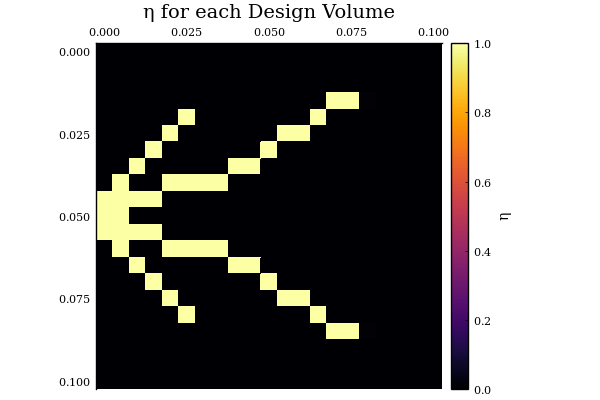
\includegraphics[width=1.1\linewidth]{Chapter_III_Implementation_and_Results/Images/20x20-Final_Design.png}
		\caption{$20\times 20$ control volumes}
		\label{fig:SIMP-Output-20}
	\end{subfigure}
	\begin{subfigure}{0.5\textwidth}
		\centering
		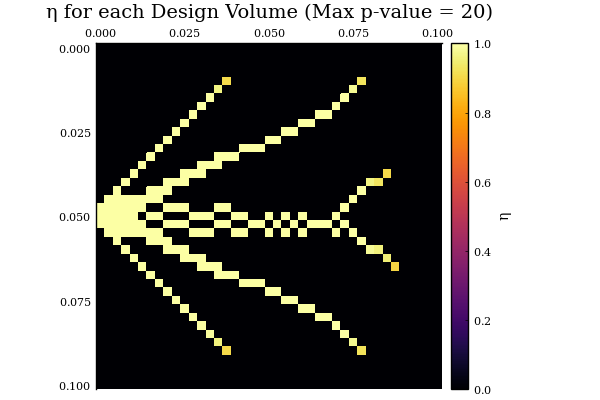
\includegraphics[width=1.1\linewidth]{Chapter_III_Implementation_and_Results/Images/40x40-Final_Design.png}
		\caption{$40\times 40$ control volumes (Max $p=20$)}
		\label{fig:SIMP-Output-40}
	\end{subfigure}\\\vspace{1em}
	\begin{center}
	\begin{subfigure}{0.75\textwidth}
		\centering
		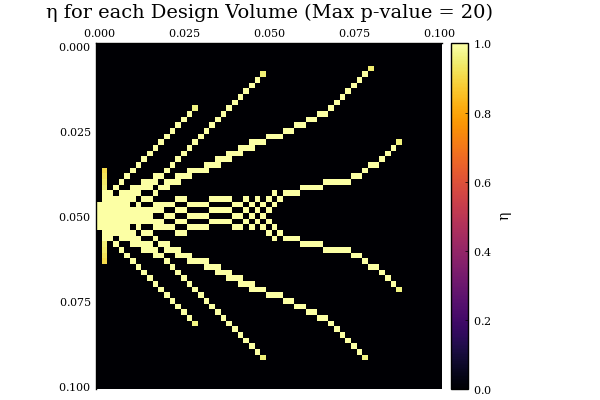
\includegraphics[width=\linewidth]{Chapter_III_Implementation_and_Results/Images/60x60-Final_Design.png}
		\caption{$60\times 60$ control volumes (Max $p=20$)}
		\label{fig:SIMP-Output-60}
	\end{subfigure}
	\end{center}
	\caption[Designs for Varying Numbers of Control Volumes]{Final design outputs of SIMP algorithm for domains with varying numbers of control volumes.}
	\label{fig:SIMP-Outputs-20-40-60}
\end{figure}
\end{center}

\begin{figure}
	\centering
	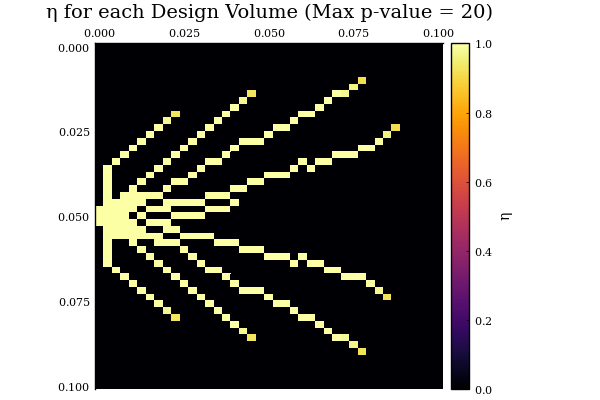
\includegraphics[width=0.75\linewidth]{Chapter_III_Implementation_and_Results/Images/50x40-Final_Design.png}
	\caption[Rectangular Control Volume Design]{$50\times 40$ control volumes (Max $p=20$)}\label{fig:SIMP-Output-50-40}
\end{figure}

Notice the alternating pattern in the conductivities of control volumes at the center of Figure \ref{fig:SIMP-Output-60}. This phenomenon is known as ``checkerboarding'' and is a consequence of our discretization scheme.

\subsection{``King Me'': Avoiding the Checkerboard Problem}\label{sec:checkerboarding}

If one were to optimize conductive material placement to increase heat transfer on a standard rectangular grid, a simplistic solution would be to create a grid of alternating material types in each adjacent rectangle, like a checkerboard. This way, the heat is always flowing to adjacent cells. While this may indeed increase heat transfer, it doesn't necessarily decrease the average temperature in our object (or transfer the heat towards the heat-sink). Hence, avoiding this non-physical checkerboard solution is of concern.

\begin{figure}
	\centering
	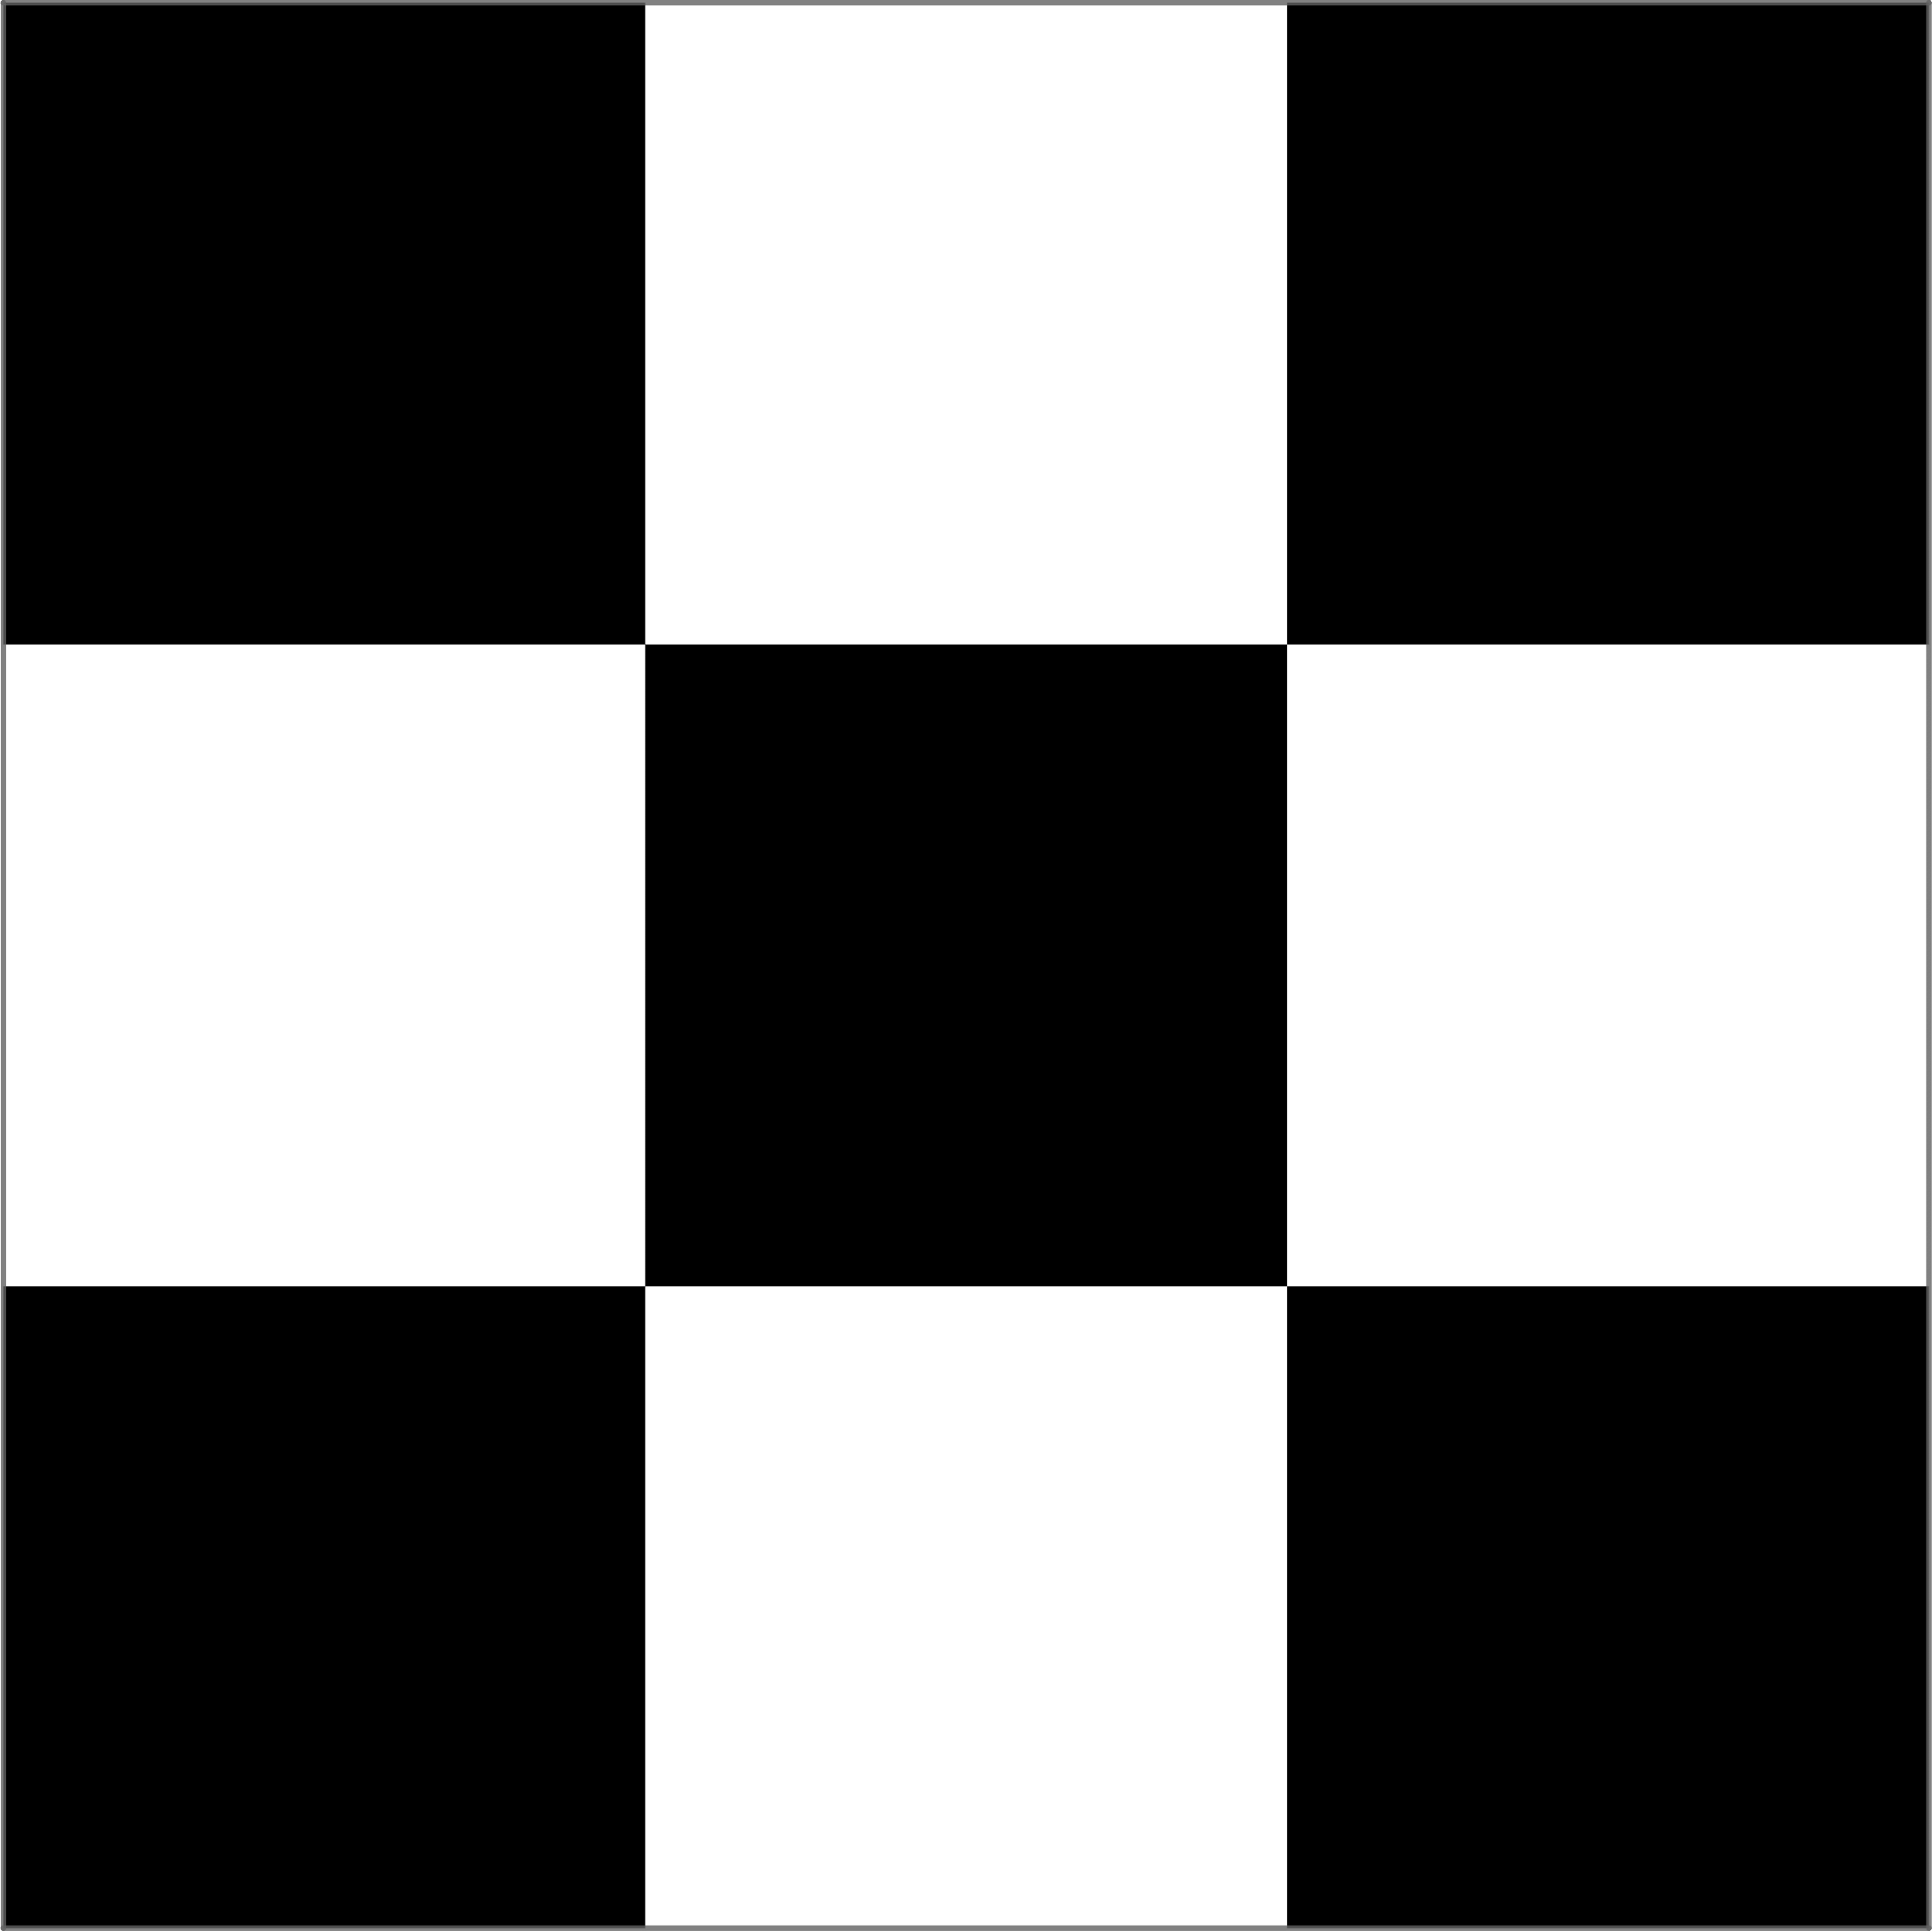
\includegraphics[width=0.4\textwidth]{Chapter_III_Implementation_and_Results/Images/3x3-Checkerboard.png}
	\caption[Checkerboard Pattern]{A checkerboard pattern result on a 3-by-3 control volume grid. The black spaces represent areas where $\eta=1$ and the white spaces represent areas where $\eta=0$ in \eqref{eqn:penalization}. This design results in adjacent regions of alternating thermal conductivites $k_+$ and $k_0$, artificially maximizing heat transfer between control volumes.}
	\label{fig:3x3-Checkerboard}
\end{figure}

\begin{figure}
	\centering
	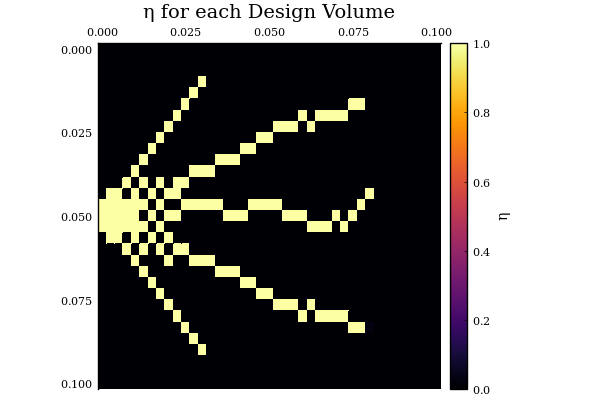
\includegraphics[width=0.8\textwidth]{Chapter_III_Implementation_and_Results/Images/SIMP-Example-Checkerboarding.png}
	\caption[Checkerboard Result in Practice]{Output of SIMP algorithm for $30\times 40$ temperature control volumes. Notice the local checkerboarding around $(0.05,0.015)$.}
	\label{fig:SIMP-Checkerboard}
\end{figure}

In order to solve the heat equation \eqref{eqn:HeatEq}, we employ the Finite Volume Method (described earlier). This involves splitting up our space into a finite number of control volumes. The checkerboard pattern emerges when the solution of our optimization process converges to a 1---0 structure which has some meshes that successively belong to the $\Omega_0$ and $\Omega_+$ sets (i.e.: adjacent grid volumes have alternating thermal conductivites). As a result, the heat transfer within the structure between $k_+$ and $k_0$ regions is maximized, artificially increasing the impact of adding $k_+$ material on the temperature $T$, which in turn minimizes the objective function in \eqref{SIMP-Optimization-Problem} \cite{Versteeg2007}. Typically, this pattern occurs locally but then spreads throughout the entire structure through successive iterations of the optimization process. However, in the real world, these checkerboard placements of our conductive materials do not actually have the effect of lowering the average temperature in structures. In fact, the checkerboard example in Figure \ref{fig:3x3-Checkerboard} doesn't even direct heat towards the heat-sink on the left wall of the structure.

In order to avoid obtaining checkerboard solutions from our optimization process, we employ two separate staggered grids for our temperature and design variables (see Figure \ref{fig:grids}). We need to employ some extra equations in order to translate between design and temperature variables, but this strategy helps solve the issue of convergence to checkerboard solutions.

Available literature on topology optimization propose other solutions as well, such as using a weighted average over neighboring nodes when finding design sensitivies and introducing constraints on the norm of the design gradients \cite{Sigmund1998}. These are methods that would be of interest to implement in future work.

\subsection{Algorithm Results}

In our implementation, the algorithm is initialized with $\eta=0.05$ for each control volume, the maximal porosity $\overline{\phi}$ was $10\%$, and $p$ was increased in steps of $0.05$ beginning at $p=1$ for each outer-loop iteration. We can see in Figure \ref{fig:60x60-p=1} that after one outer-loop iteration, the algorithm has already zeroed the design parameters for many of the control volumes.

\begin{figure}
	\centering
	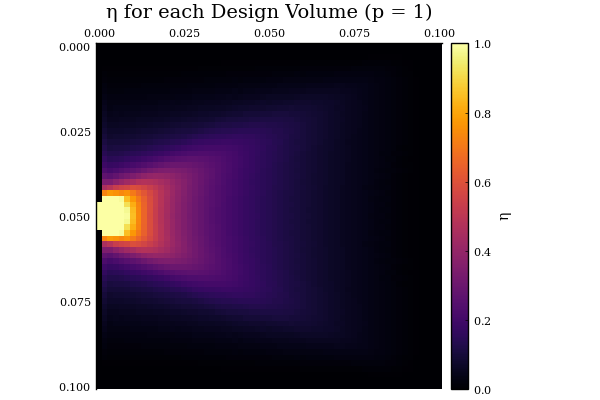
\includegraphics[width=0.75\linewidth]{Chapter_III_Implementation_and_Results/Images/60x60_1p.png}
	\caption[One Outer-Loop Iteration]{Design after one outer-loop iteration for a $60\times 60$ control volumes.}
	\label{fig:60x60-p=1}
\end{figure}

With each outer-loop iteration and increasing $p$, the objective function values for the average temperature increases quite rapidly until it begins to level off. For a $60\times 60$ control volume design, the temperature values begin to converge around $p=5$ (Figure \ref{fig:p-vs-T}). The increase in temperature is due to concentration of the $k_+$ material and penalizing fractional portions of $\eta$.

\begin{figure}
	\centering
	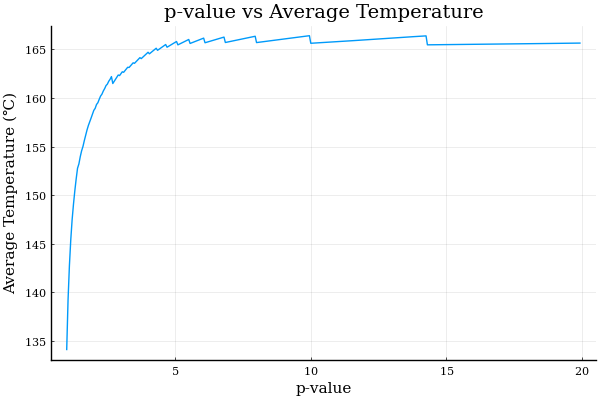
\includegraphics[width=0.75\linewidth]{Chapter_III_Implementation_and_Results/Images/60x60-p_vs_T.png}
	\caption[$p$-value vs. $T_{av}$]{$p$-value plotted against Average Temperature Evaluation for $60\times 60$ control volumes with a maximum $p$-value of $20$.}
	\label{fig:p-vs-T}
\end{figure}

In general, the number of inner loop iterations seems to quickly decrease as $p$ increases, but there are fluctuations that occur occasionally (Figure \ref{fig:p-vs-Inner-Itter}). It is not clear as to why the inner-loop converges after a small number of iterations (often 2 or 3) for one $p$-value and then will require over $100$ iterations for a following $p$-value. Other literature on the VP heat conduction problem did not have an explanation for this behavior either \cite{Marck2012}.

\begin{figure}
	\begin{center}
	\begin{subfigure}{0.8\textwidth}
		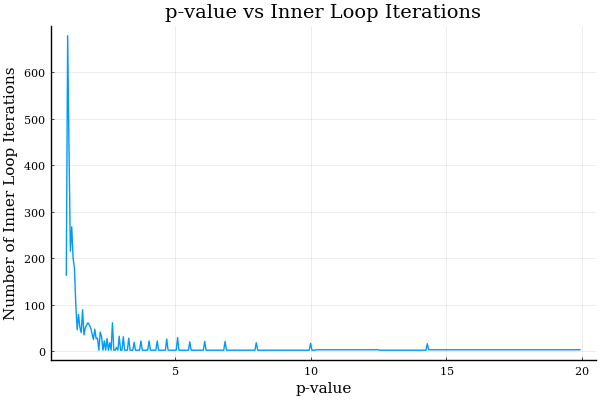
\includegraphics[width=\linewidth]{Chapter_III_Implementation_and_Results/Images/60x60-p_vs_Inner-Itter.png}
		\caption[$p$-value vs. $T_{av}$]{$p$-value plotted against the number of inner loop iterations for $60\times 60$ control volumes with a maximum $p$-value of $20$.}
		\label{fig:p-vs-Inner-Itter-60x60}
	\end{subfigure}
	\end{center}
	\vspace{1em}
	\begin{center}
	\begin{subfigure}{0.8\textwidth}
		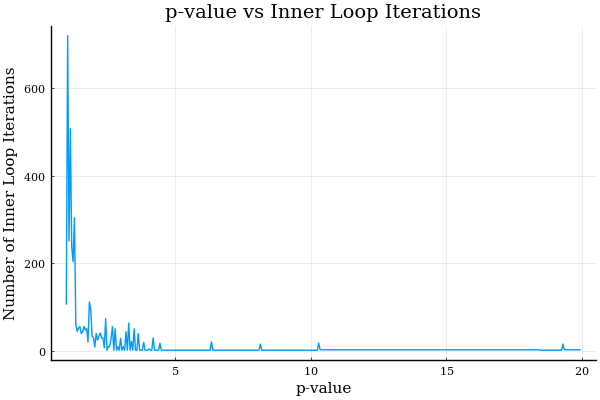
\includegraphics[width=\linewidth]{Chapter_III_Implementation_and_Results/Images/50x40-p_vs_Inner-Itter.png}
		\caption[$p$-value vs. $T_{av}$]{$p$-value plotted against the number of inner loop iterations for $50\times 40$ control volumes with a maximum $p$-value of $20$.}
		\label{fig:p-vs-Inner-Itter-50x40}
	\end{subfigure}
	\end{center}
	\caption[$p$-value vs. Number of Inner Loop Iterations]{$p$-value vs. Number of Inner Loop Iterations for Square and Rectangular Control Volumes}
	\label{fig:p-vs-Inner-Itter}
\end{figure}

It is interesting to note that the fluctuations in the number of inner-loop iterations seem to be of greater magnitude for the rectangular control volume examples tested. (See Figure \ref{fig:p-vs-Inner-Itter-60x60} versus Figure \ref{fig:p-vs-Inner-Itter-50x40}.)

The algorithm was also run with high initial $p$-values. Rather than starting with $p=1$, Figure \ref{fig:start_p=5} shows the resulting design for initializing the algorithm with $p=5$. In this case, the algorithm converged very quickly: one outer-loop iteration. In this case, the algorithm determines that it is best to densely place the expensive $k_+$ material around the heatsink. If the initial penalization parameter is too high, the algorithm appears to stall at the initial guess. In Figure \ref{fig:start_p=19} the algorithm was initialized with $p=19$. Here, the algorithm ran 3 outer-loop iterations, but the final design is the same as the initial input design. It appears that with such a high penalization parameter it costs too much to change the conductivity at any control volume and the solution the optimizer outputs is the initial guess.

\begin{figure}
	\begin{subfigure}{0.5\textwidth}
		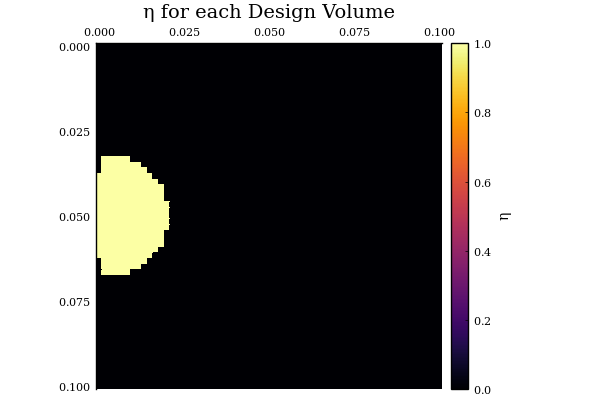
\includegraphics[width=1.1\linewidth]{Chapter_III_Implementation_and_Results/Images/60x60-start-p=5-1iters.png}
		\caption{$60\times 60$ Control Volumes with Initial $p=5$.}
		\label{fig:start_p=5}
	\end{subfigure}
	\begin{subfigure}{0.5\textwidth}
	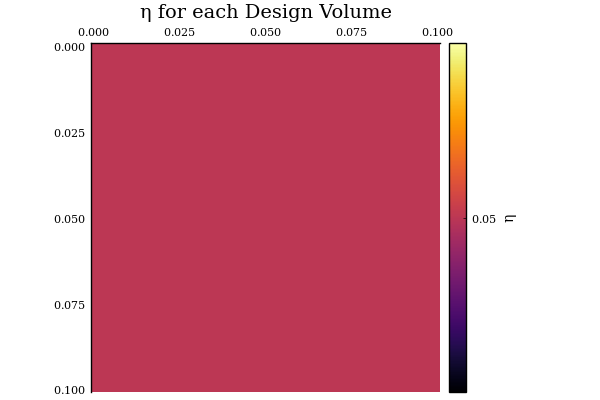
\includegraphics[width=1.1\linewidth]{Chapter_III_Implementation_and_Results/Images/60x60-start-p=19-3iters.png}
	\caption{$60\times 60$ Control Volumes with Initial $p=19$.}
	\label{fig:start_p=19}
\end{subfigure}
\caption[Designs with Higher Initial $p$]{SIMP Algorithm design outputs for inital $p$-values greater than $1$.}
\end{figure}

For the designs tested, it appears that the total algorithm runtime increases quadratically with the total number of control volumes in the design (Figure \ref{fig:runtime}).

\begin{figure}
	\centering
	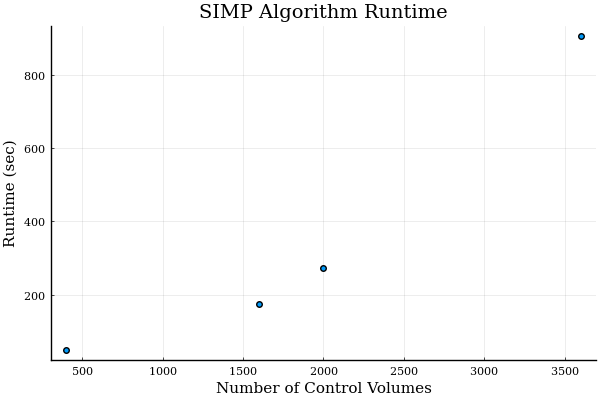
\includegraphics[width=0.8\linewidth]{Chapter_III_Implementation_and_Results/Images/SIMP-Runtime.png}
	\caption[SIMP Runtime Plot]{Plot of runtime for SIMP algorithm for various numbers of control volumes.}
	\label{fig:runtime}
\end{figure}